\documentclass[a4paper]{article}
\usepackage[left=1.0in,top=1.0in,right=1.0in,bottom=1.0in]{geometry}
\usepackage[english]{babel}
\usepackage[utf8]{inputenc}
\usepackage{hyperref,graphicx}
\usepackage{
  amssymb,
  amsmath,
  amsthm,
  latexsym
}
\graphicspath{{./images/}}
\title{Lab 3 Oscilloscope}
\author{Philip Kim}
\date{\today}
\begin{document}
\maketitle
\begin{center}
  \section*{1. The oscilloscope and function generator}
  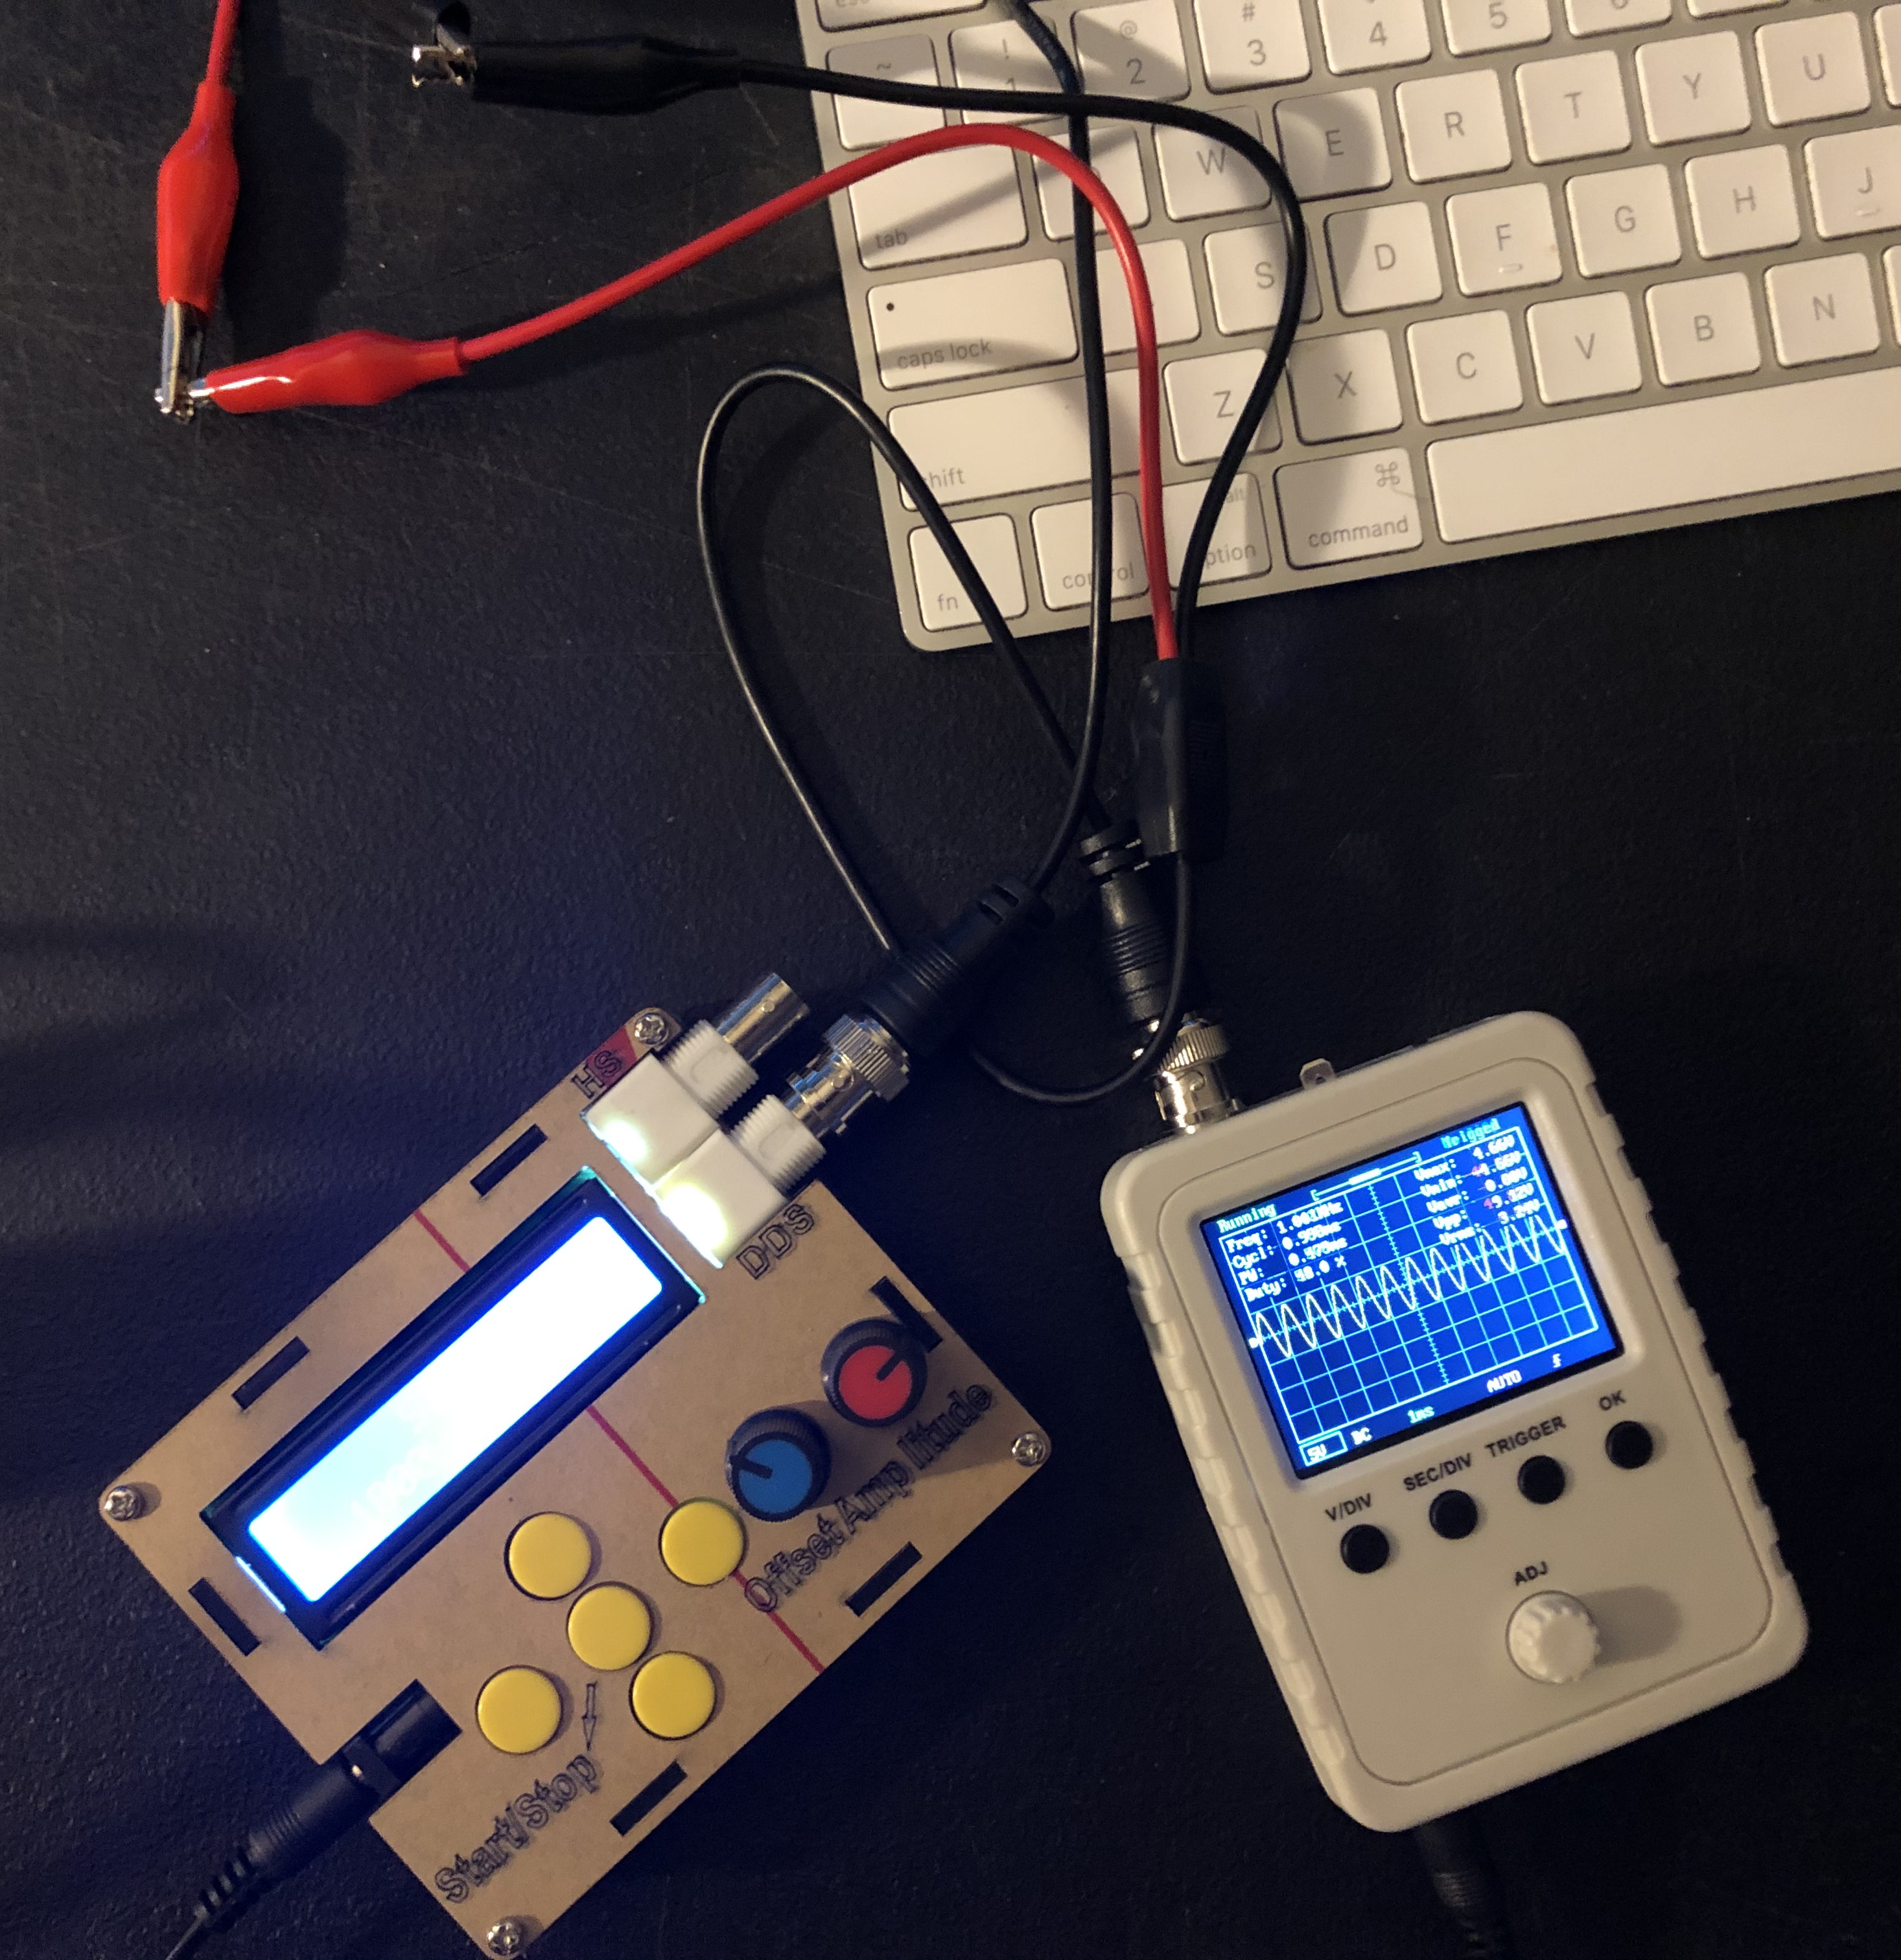
\includegraphics[scale=0.08]{1.jpeg}
  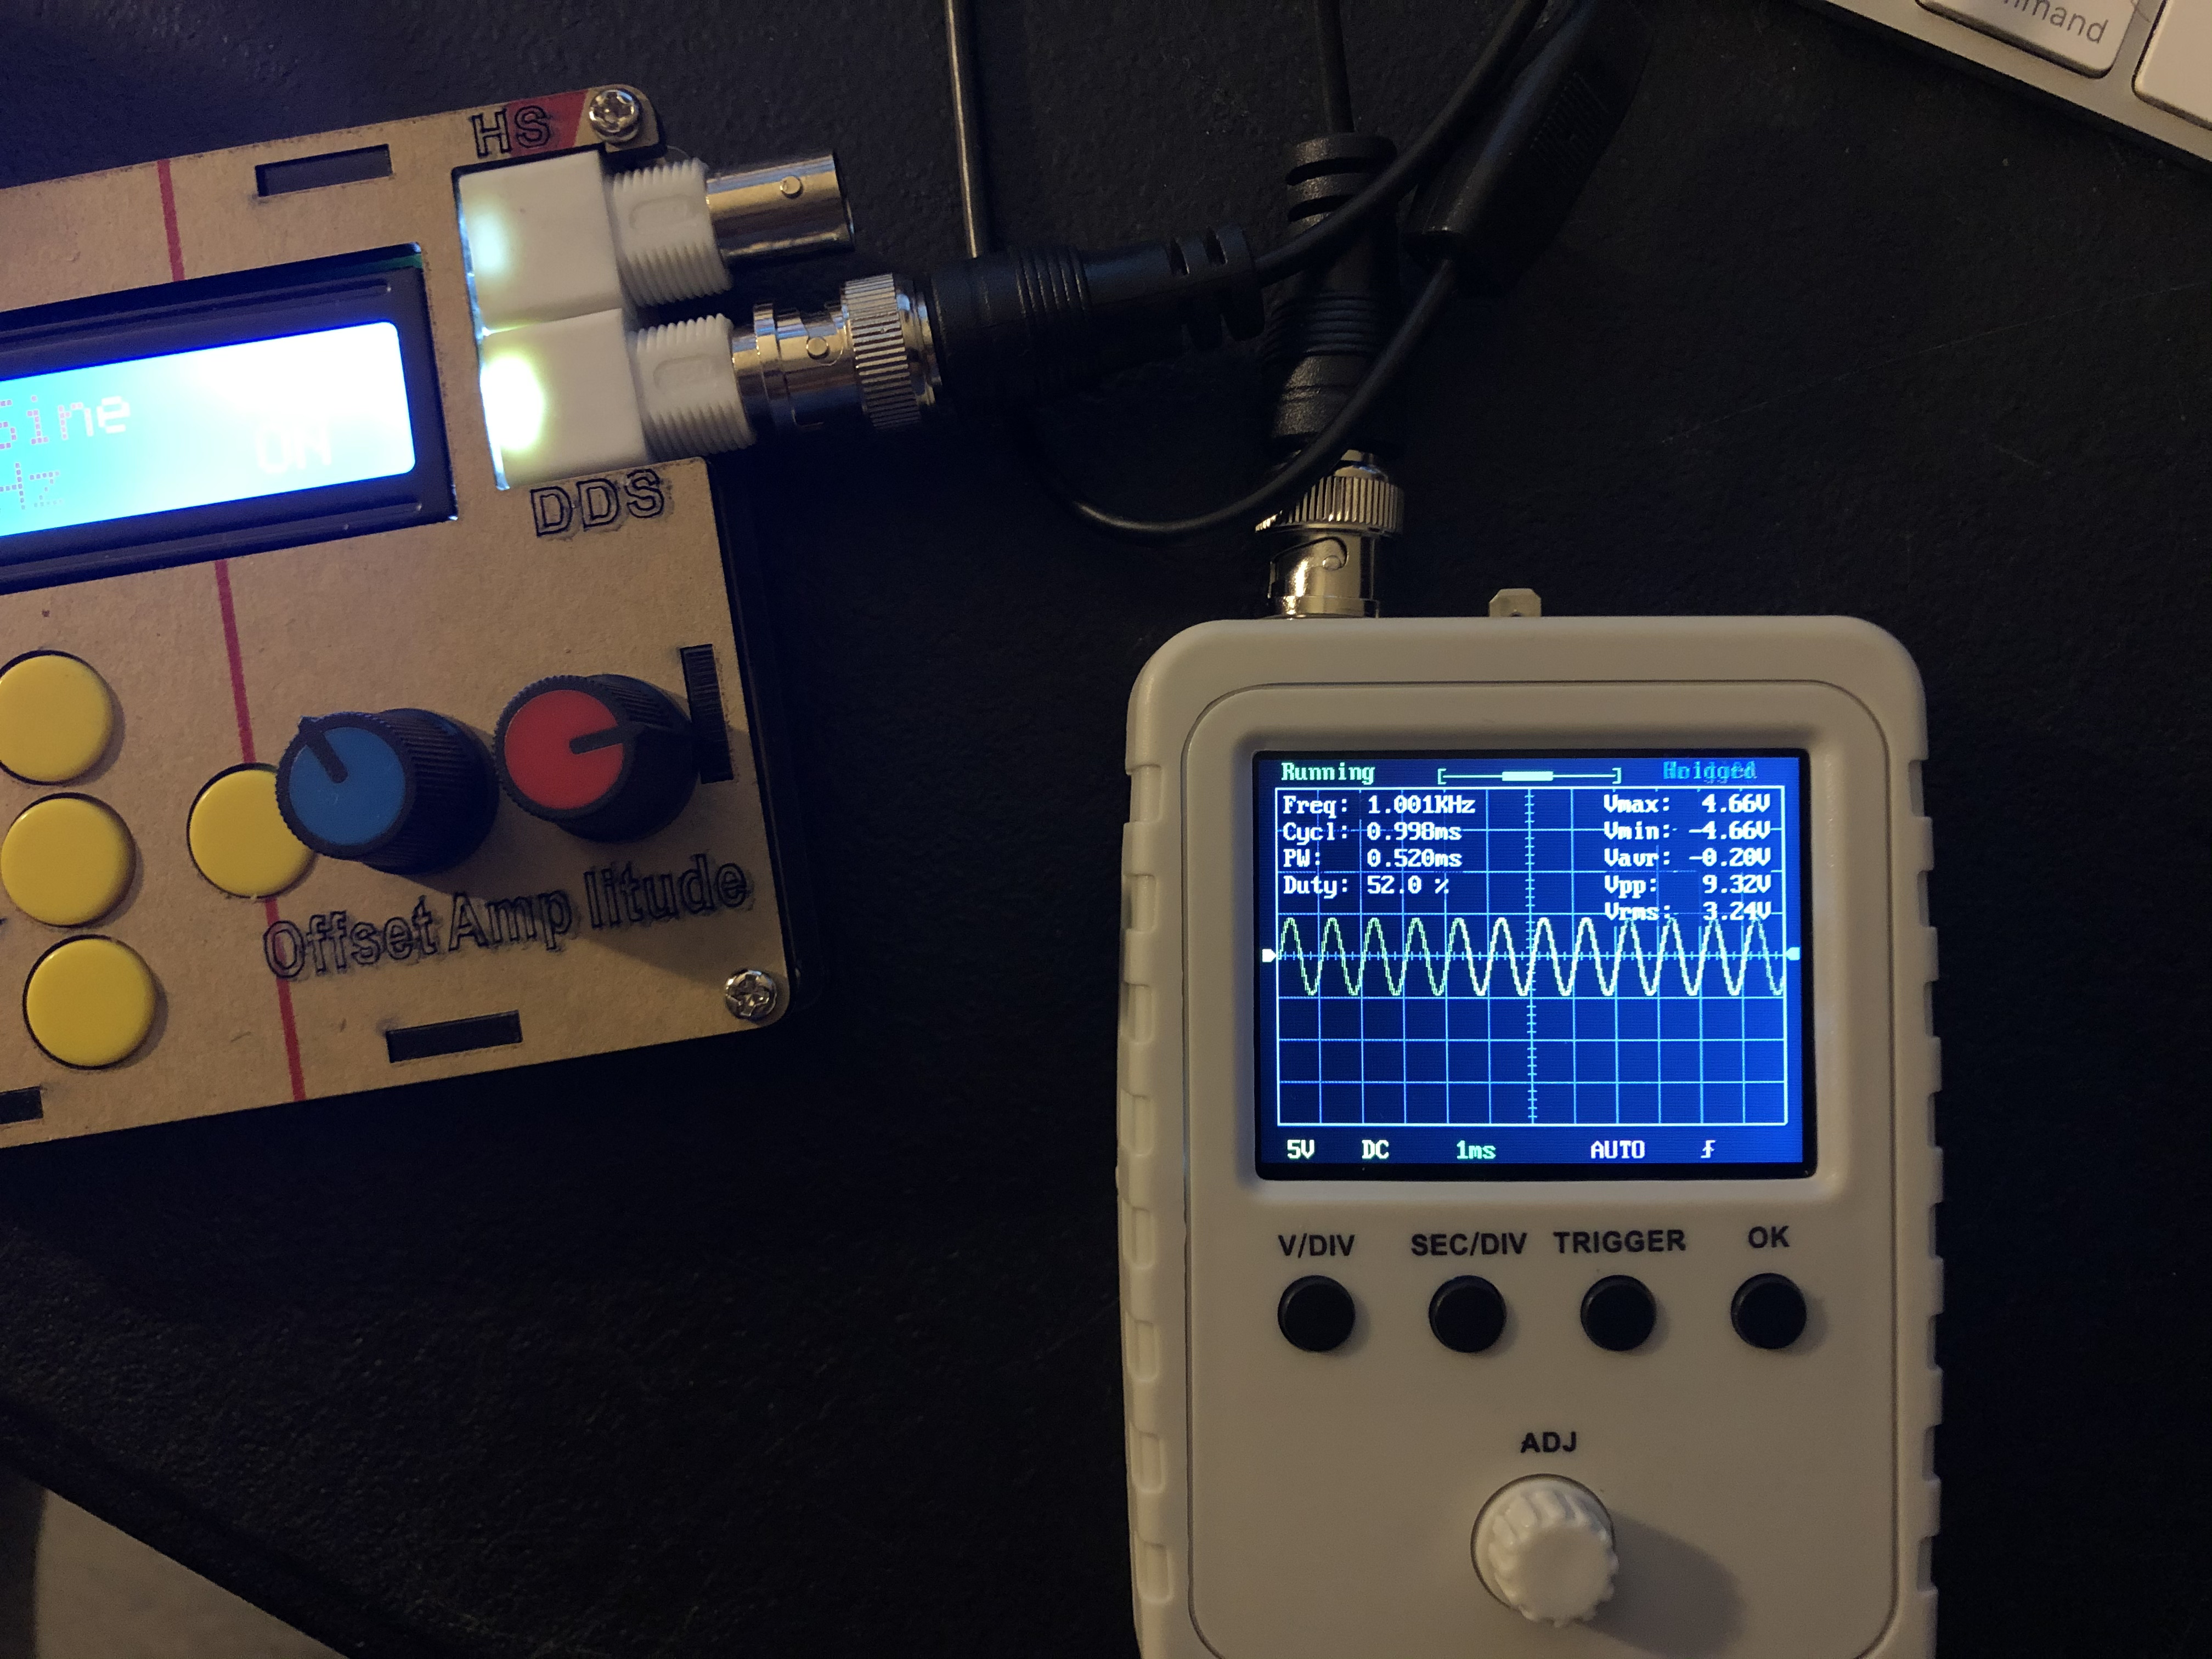
\includegraphics[scale=0.08]{1a.jpeg}
\end{center}
\newpage
\begin{center}
  \section*{2. The resistor and capacitor organization}
  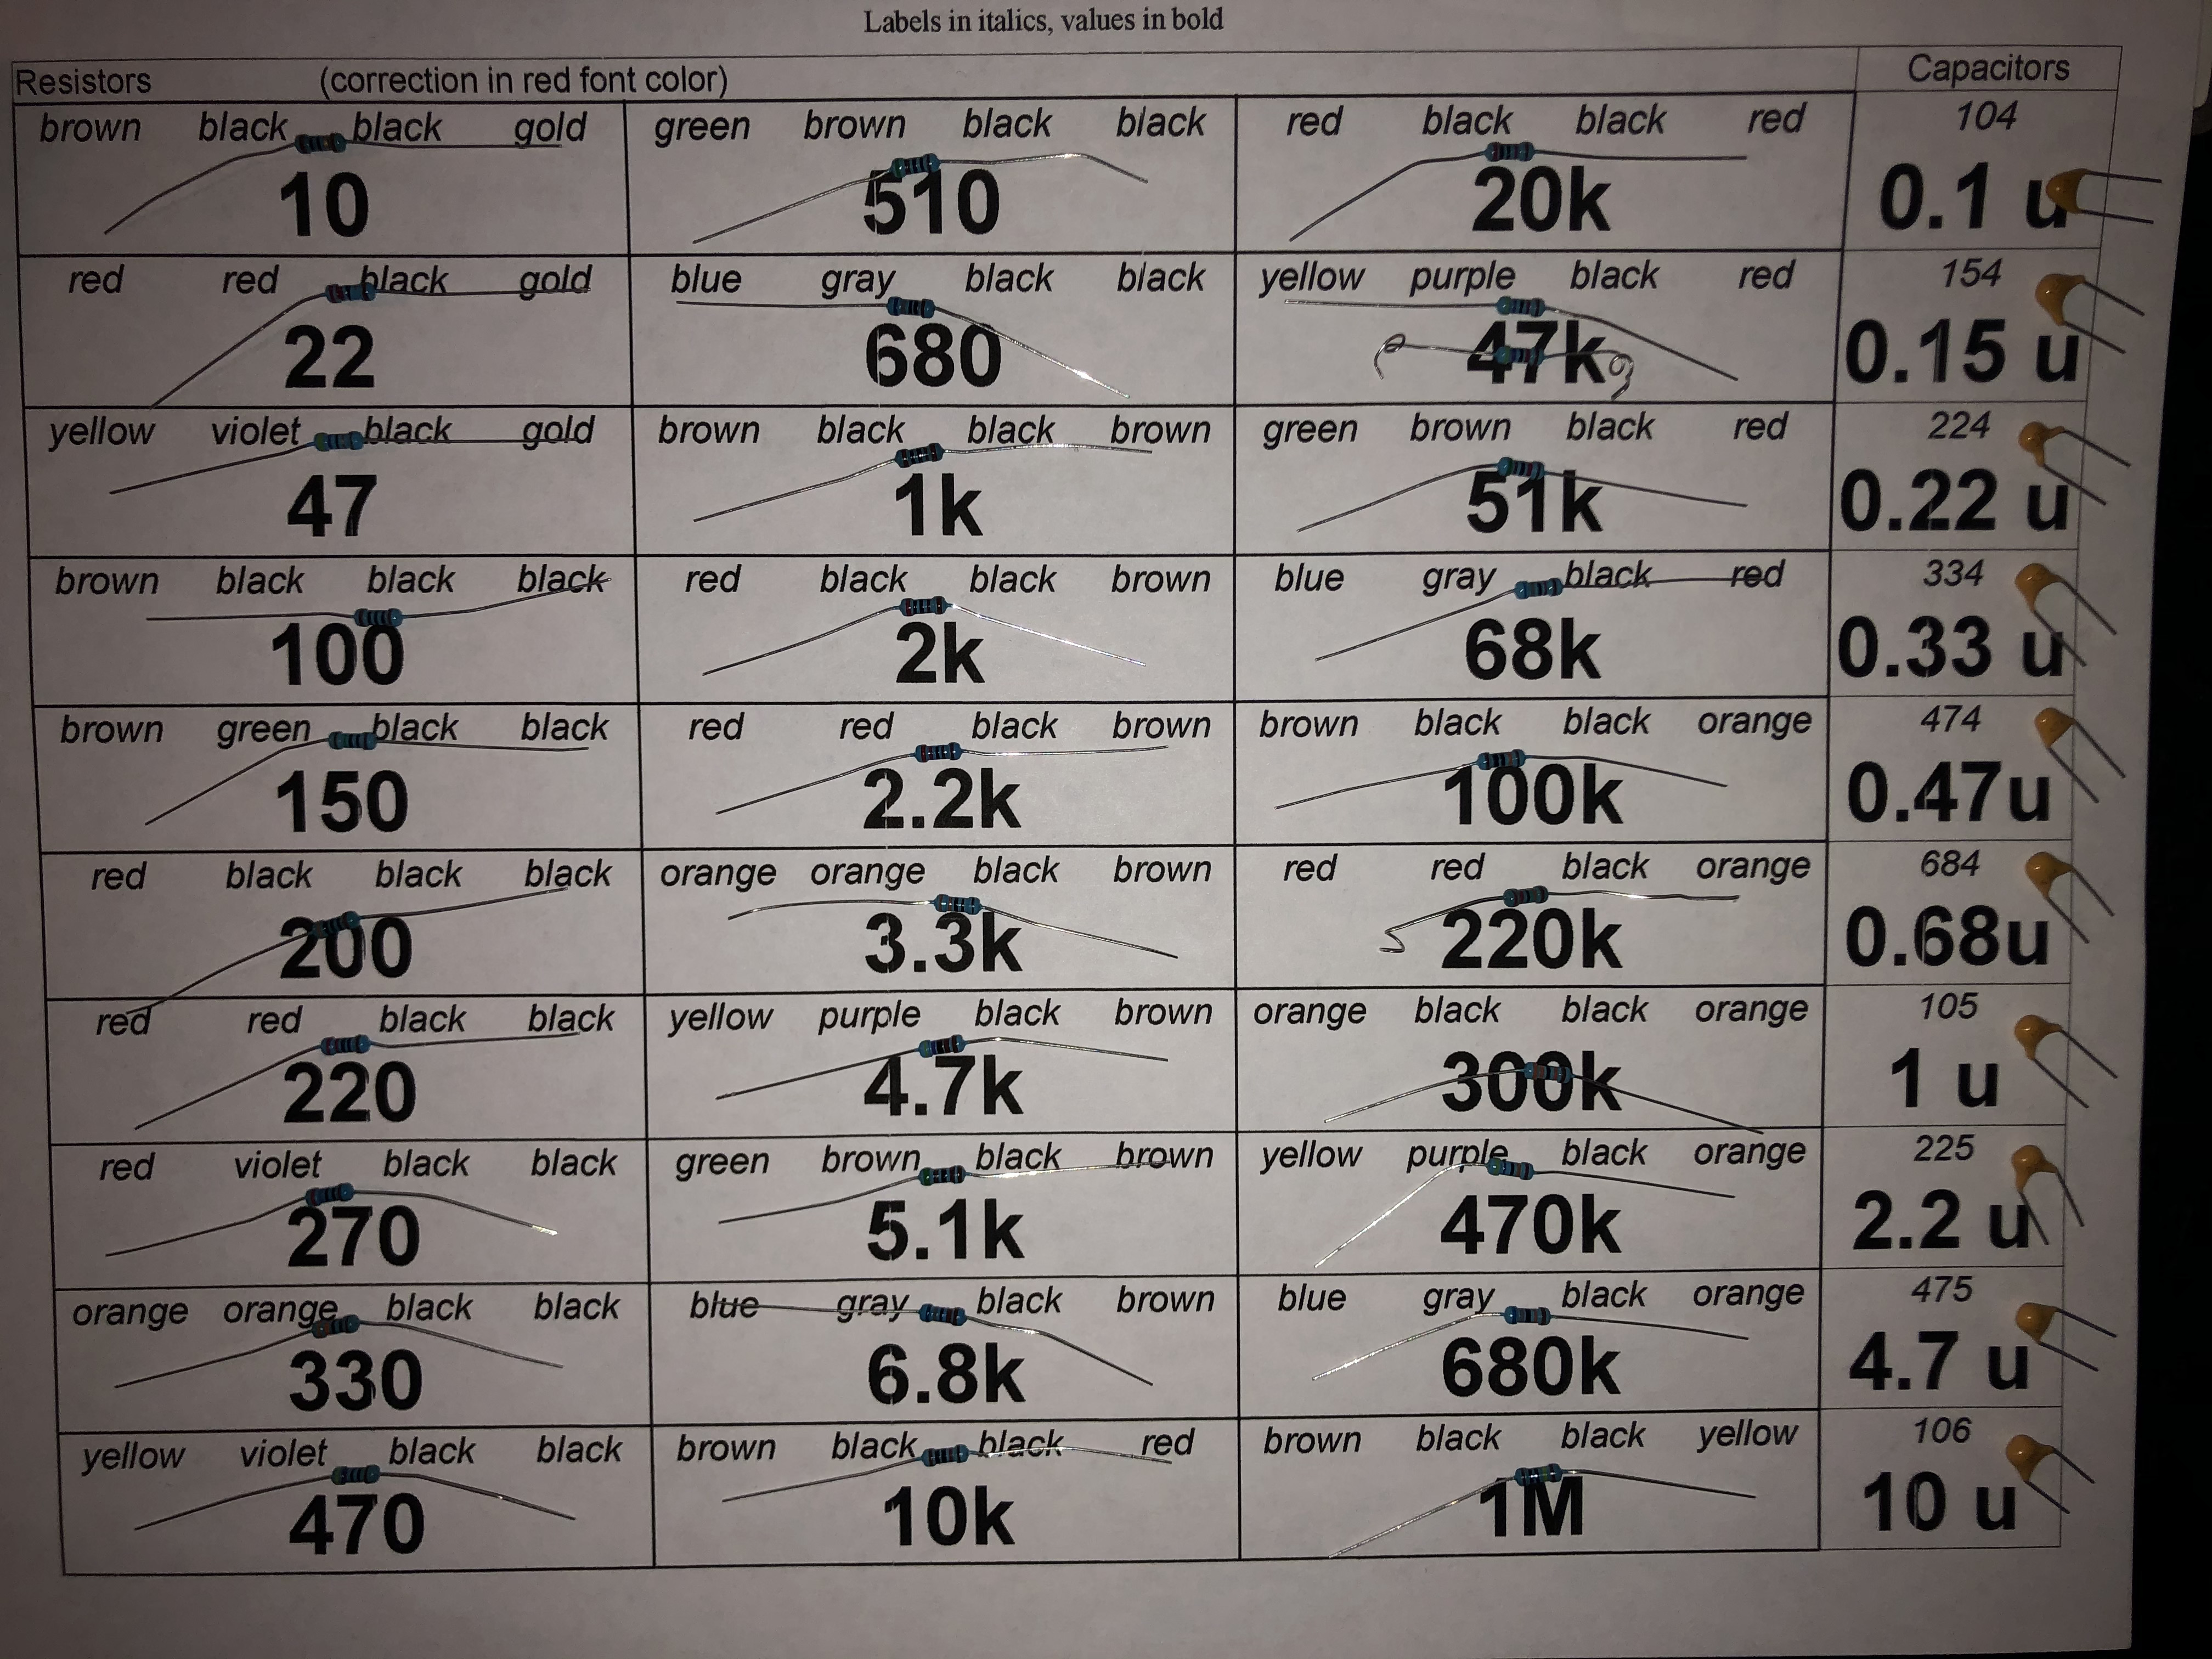
\includegraphics[scale=0.08]{2.jpeg}
  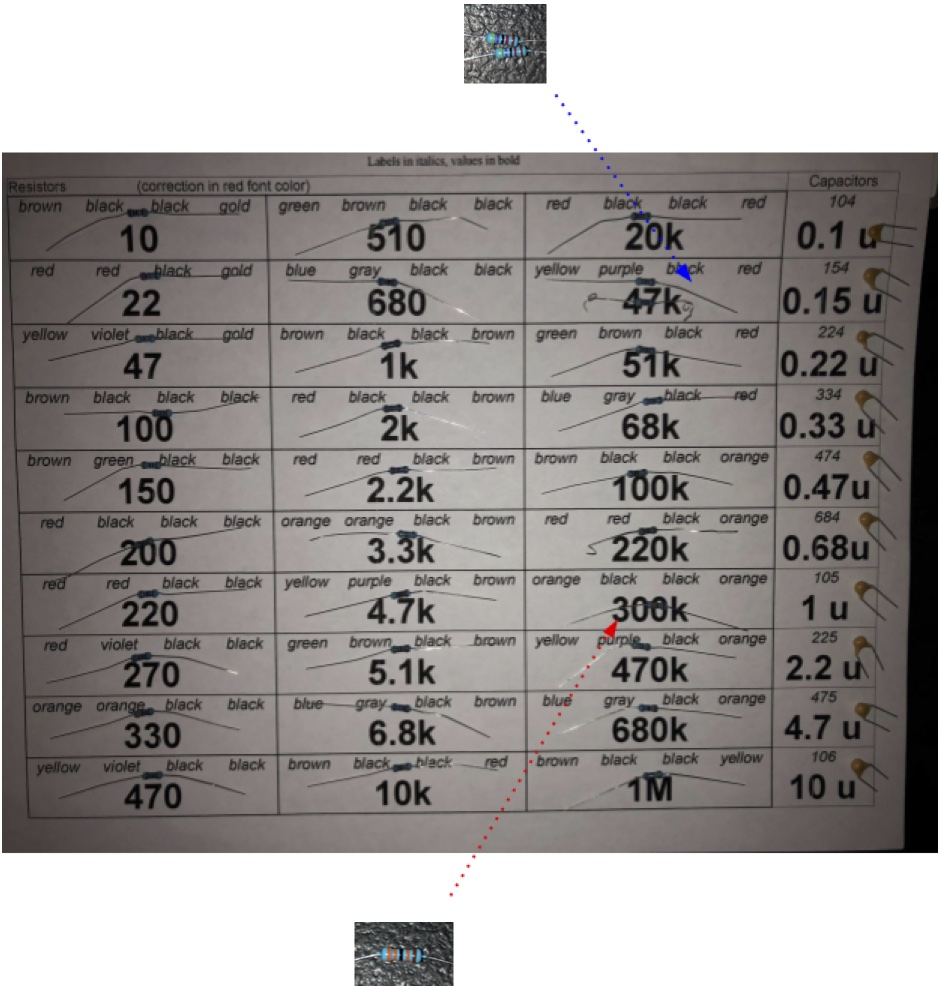
\includegraphics[scale=0.4]{2a.jpg}
\end{center}
\begin{itemize}
  \item \textbf{47k\(\Omega \)}: Yellow, purple, black, red for both resistors.
  \item \textbf{300k\(\Omega \)}: Orange, orange, black, orange for only resistor not matching.
\end{itemize}
\end{document}
% 47k,300k